\documentclass[a4paper, 12pt, finnish]{article}
\usepackage{babel}
\usepackage{afterpage}
\usepackage[utf8]{inputenc}
\usepackage[T1]{fontenc}
\usepackage{amsmath}
\usepackage[margin=0.9in]{geometry}
\geometry{a4paper}
\usepackage{graphicx}
\usepackage{float}
\usepackage{wrapfig}
\usepackage{caption}
\usepackage{eurosym}
\usepackage[section]{placeins}
\usepackage{url}
\usepackage[hidelinks]{hyperref}
\usepackage{hyperref}
\usepackage{subcaption}
\usepackage{lipsum}
\usepackage{changepage}
\usepackage{bookmark}
\usepackage[table,xcdraw]{xcolor}
\usepackage[export]{adjustbox}
\definecolor{grey}{rgb}{0.9,0.9,0.9}
\def\UrlBreaks{\do\/\do-}
\graphicspath{{./figures/}}
\begin{document}
\begin{titlepage}
	\colorbox{grey}{
		\parbox[t]{0.93\textwidth}{
			\parbox[t]{0.91\textwidth}{
				\raggedleft
				\fontsize{80pt}{80pt}\selectfont
				\vspace{0.7cm}
				\textbf{MX Linux 18\\
				käyttöopas\\}
				\vspace{0.7cm}
			}
		}
	}
	\vfill
	\parbox[t]{0.93\textwidth}{
		\raggedleft
		\large
		{\Large Iiro Aarnio}\\[4pt]
		Projektissa toimiminen\\
		Tampereen seudun ammattiopisto\\[4pt]
		\url{github.com/maysion/mxlinux18}\\
		\hfill\rule{0.2\linewidth}{1pt}
	}
\end{titlepage}
\thispagestyle{empty}
\begin{abstract}
	Tässä käyttöoppaassa perehdytään MX Linux 18 -GNU/Linux-jakelun käyttöönottoon ja käyttöön. Käyttöopas on suunnattu henkilöille, joilla ei ole aiempaa kokemusta Linux-järjestelmistä. Käyttöopas sisältää muun muassa käyttöjärjestelmän asentamisen, ohjelmien hakemisen ja päivittämisen. Opas ei sisällä laitteiston valmistelua.
\end{abstract}

\newpage
\thispagestyle{empty}
\tableofcontents
\newpage
\pagenumbering{arabic}
\setcounter{page}{1}
\newpage

%%% DOC

\section{Mikä on MX Linux 18?}
MX Linux 18 on työpöytäkäyttöön tarkoitettu GNU-käyttöjärjestelmään pohjautuva jakelu. Puhekielessä näistä jakeluista puhutaan usein Linux-käyttöjärjestelminä. Tässä oppaassa käytetään oikeaoppista termiä, GNU/Linux-jakelu.

MX Linux 18 perustuu tunnetumpaan GNU/Linux-jakeluun nimeltä Debian. Sadat eri käyttöjärjestelmät perustuvat Debian-jakeluun, sillä se on vakaa ja suhteellisen helposti muokattavissa käyttäjäystävälliseksi.

\subsection{Miten MX Linux 18 eroaa muista käyttöjärjestelmistä?}
MX Linux 18 eroaa monin eri tavoin muista markkinoilla olevista käyttöjärjestelmistä, sillä se pohjautuu GNU-käyttöjärjestelmään ja hyödyntää Linux-ydintä.

Työpöytäkäytössä GNU/Linux-järjestelmien edut ovat huomattavat. Suuri osa GNU/Linux-jakeluista ovat todella kevyitä ja toimivat hyvin vanhemmalla laitteistolla. Markkinoiden suosituimmat käyttöjärjestelmät, Microsoft Windows sekä MacOS, ovat todella raskaita käyttöjärjestelmiä ja vaativat suhteellisen uutta laitteistoa. MX Linux 18 on kevyt ja suunniteltu toimivaksi mahdollisimman monilla erilaisella laitteistolla.

\section{Asennus}
\subsection{Asennusmedian käynnistäminen}
MX Linux 18 -jakelun käynnistyttyä käynnistysmedialta, avautuu kuvanmukainen valikko. (Kuva \ref{fig:boot})
Painamalla F2-näppäintä, voidaan valita haluttu kieli. Valintaa voi muokata nuolinäppäimillä. (Kuva \ref{fig:lang}) Kieliasetus on hyvä määrittää tässä vaiheessa, sillä se määrittää koko asennusprosessin kielen.

\begin{figure}[htbp]
     \centering
      \begin{minipage}{.5\textwidth}
           \centering
            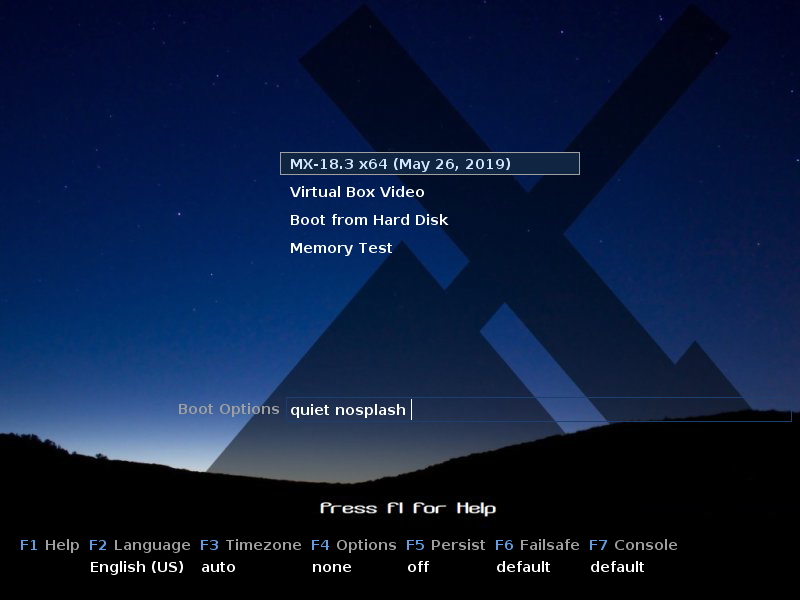
\includegraphics[width=.98\linewidth]{asen/boot}
             \captionof{figure}{Käynnistysvalikko}
              \label{fig:boot}
               \end{minipage}%
               \begin{minipage}{.5\textwidth}
                    \centering
                     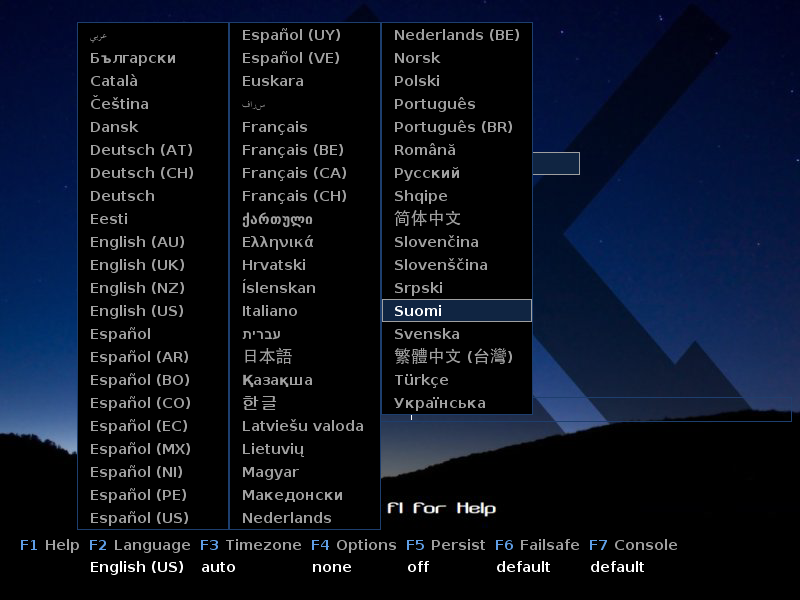
\includegraphics[width=.98\linewidth]{asen/lang}
                      \captionof{figure}{Käynnistysvalikon kieliasetukset}
                       \label{fig:lang}
                        \end{minipage}
                         \end{figure}


Kielen valitsemisen jälkeen jakelun voi käynnistää niin kutsuttuun livetilaan, painamalla Enter-painiketta.

\subsection{Livetila}

Toisin kuin yleisimmät kaupalliset käyttöjärjestelmät, GNU/Linux-jakelut käynnistyvät usein nk. livetilaan, josta jakelu asennetaan.
Livetilassa voi tarkastella järjestelmän ja kovalevyjen tietoja. Mikään tallennettu tiedosto ei kuitenkaan säily käynnistysten välissä. Livetilaa voi hyödyntää esimerkiksi yksityisyyden korostamiseen, tietokoneen korjaamiseen tai jakeluun tutustumiseen ilman varsinaista asennusta. Jakelun käynnistyttyä livetilaan ruudulle ilmestyy Tervetulo-ohjelma.
Tervetulo-ohjelmasta löytyy paljon hyödyllistä tietoa jakelusta ja sen käytöstä. (Kuva \ref{fig:welcome})

\begin{figure}[htpb]
    \begin{center}
        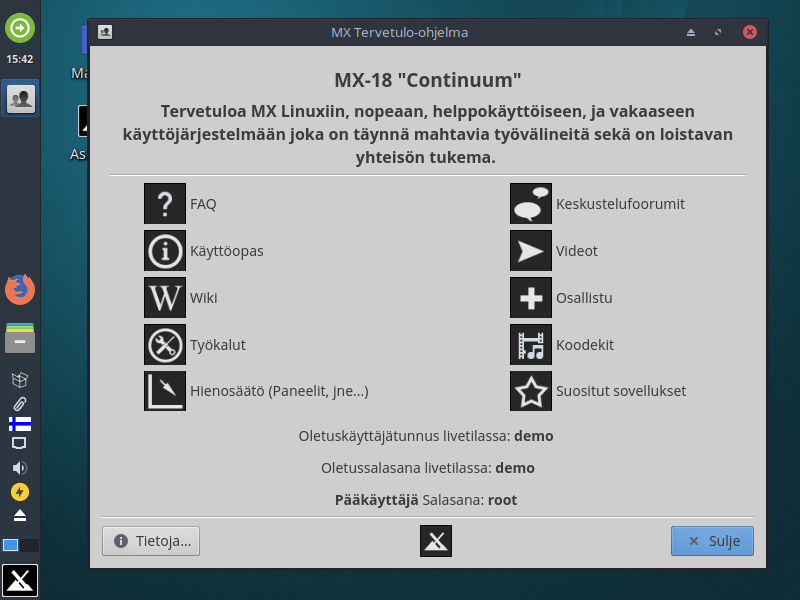
\includegraphics[width=0.9\textwidth]{asen/welcome}
        \caption{Tervetulo-ohjelma}
        \label{fig:welcome}
    \end{center}
\end{figure}

\subsection{Asennuksen aloittaminen}

Aloittaaksesi asennuksen, sulje kaikki muut sovellukset ikkunoiden oikeasta yläkulmasta. Paikanna asennusohjelma työpöydältä ja avaa se tuplaklikkaamalla sitä kursorilla. (Kuva \ref{fig:asenna}) Tämän jälkeen asennusohjelma käynnistyy ja asennus voidaan aloittaa tarpeellisten määritysten jälkeen.

\begin{figure}[htpb]
    \begin{center}
        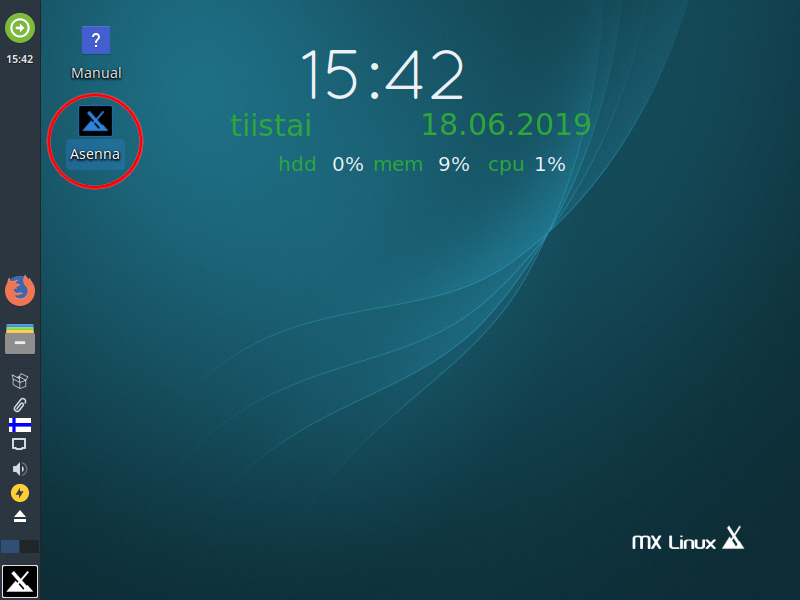
\includegraphics[width=0.875\textwidth]{asen/asenna}
        \caption{Asennusohjelman pikakuvake ympyröitynä}
        \label{fig:asenna}
    \end{center}
\end{figure}

\subsection{Asennusohjelma}

Asennusohjelma käynnistyy perinteisenä ikkunana. Tässä ikkunassa tehdään kaikki tarvittavat määritykset ja lopuksi asennetaan jakelu kovalevylle.

Ensimmäisessä vaiheessa on lyhyt esittelyteksti sekä näppäimistöasetusten valinta. Mikäli näppäimistön asettelun kohdalla ei lue \textbf{fi}, muuta asettelua painamalla \textit{Muuta näppäimistön asetuksia}. Kun näppäimistön asettelu on vaihdettu sopivaksi, asennusta voi jatkaa painamalla Seuraava-nappia. (Kuva \ref{fig:as1})

\begin{figure}[htpb]
    \begin{center}
        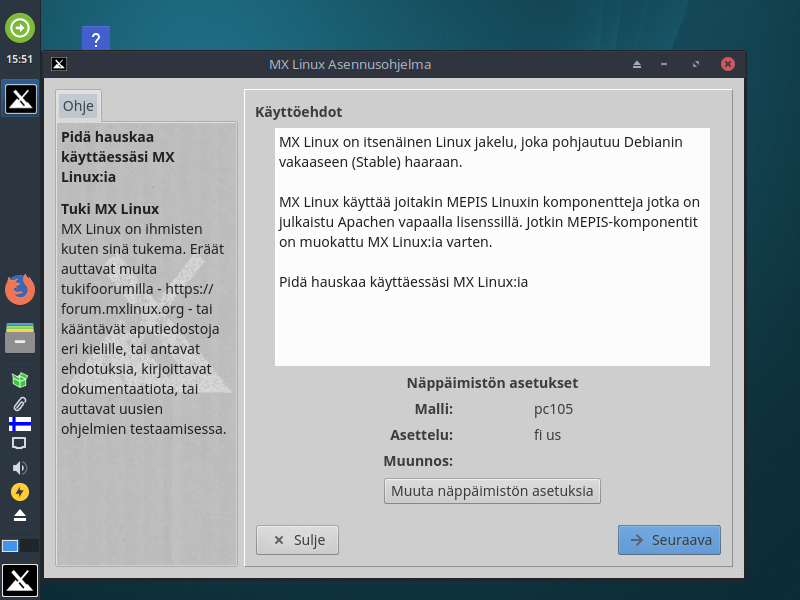
\includegraphics[width=0.875\textwidth]{asen/asennusohjelma1}
        \caption{Asennusohjelman ensimmäinen vaihe}
        \label{fig:as1}
    \end{center}
\end{figure}
\end{document}
